% We switch to portrait mode. This works as advertised.
\documentclass[a0,portrait]{a0poster}
% You might find the 'draft' option to a0 poster useful if you have
% lots of graphics, because they can take some time to process and
% display. (\documentclass[a0,draft]{a0poster})

%\usepackage[utf8]{inputenc}

% Switch off page numbers on a poster, obviously, and section numbers too.
\pagestyle{empty}
\setcounter{secnumdepth}{0}

%fonts
\usepackage[T1]{fontenc}
\usepackage{kpfonts}
%\usepackage{roboto}
\usepackage{fontspec}
%\usepackage[oldstylenums, largesmallcaps]{kpfonts}
%\setmainfont[Numbers=OldStyle]{Tex Gyre Pagella}
\setmainfont{Tex Gyre Pagella}
%\setsansfont[BoldFont=Lovelo-LineBold]{Lovelo-LineBold}
\setsansfont{Choplin-Medium-DEMO}
%\setsansfont{RobotoSlab-Bold}
%\setsansfont[StylisticSet=4]{MEgalopolisExtra}
%\renewcommand*\sfdefault{ugq}

\usepackage{hyperref}
\hypersetup{%
	pdftitle={Wrinkling and nested buckling in a confined protein gel},%the title
	pdfauthor={Mathieu Leocmach},%your name
	hidelinks=true,
}

%proper math and math symbols
%\usepackage{amsmath}
\usepackage{amssymb}

\usepackage{siunitx}

\usepackage{tabu}
\usepackage{multirow}

% Allow the usage of graphics (.jpg, .png, etc.) in the document
\usepackage{graphicx}
\usepackage{tikz}
\usetikzlibrary{arrows,shapes,backgrounds, positioning, intersections, decorations.markings, decorations.shapes, mindmap, shapes.geometric, matrix, patterns}

\usepackage{pgfplots}
\pgfplotsset{compat=1.9}
\usepackage{pgfplotstable}
%\usepgfplotslibrary{units}
\usepgfplotslibrary{groupplots}
\pgfplotsset{every axis/.append style={xlabel near ticks,ylabel near ticks,mark size={0.2em}}}
\pgfplotsset{every axis plot post/.append style={very thick}}

\usepgfplotslibrary{external}
\tikzexternalize
\tikzsetexternalprefix{fig_poster_palavas/}
\tikzset{external/system call={lualatex \tikzexternalcheckshellescape -halt-on-error -interaction=batchmode -jobname "\image" "\texsource"}}


\usepackage{ragged2e}
\RaggedRight

\definecolor{Main}{rgb}{1, 0.57, 0}
\definecolor{Accent1}{rgb}{1,0.28,0}
\definecolor{Accent2}{rgb}{1,0.74,0}

% see documentation for a0poster class for the size options here
\let\Textsize\normalsize
\def\Norulehead#1{\noindent\hbox to \hsize{\hfil\LARGE\textcolor{Main}{\textsf{#1}}}\bigskip}
\def\Head#1{\Norulehead{\dotfill #1}}
\def\LHead#1{{\LARGE #1}\smallskip}
\def\Subhead#1{\noindent{\large\color{Accent1}\textsc{#1}}}
\def\Title#1{\noindent{\VeryHuge\color{Accent2}\raggedright\textsf{\uppercase{#1}}}}

\renewcommand{\descriptionlabel}[1]{\hspace{\labelsep}\textcolor{Accent2}{\textsc{#1}}}

% The textpos package is necessary to position textblocks at arbitary 
% places on the page.
\usepackage[absolute,overlay,showboxes
]{textpos}
% Set up the grid
%
% Note that [40mm,40mm] is the margin round the edge of the page --
% it is _not_ the grid size. That is always defined as 
% PAGE_WIDTH/HGRID and PAGE_HEIGHT/VGRID. In this case we use
% 15 x 25. This gives us a wide central column for text (7 grid
% spacings) and two narrow columns (3 each) at each side for 
% pictures, separated by 1 grid spacing.
%
% Note however that texblocks can be positioned fractionally as well,
% so really any convenient grid size can be used.
%
\TPGrid[40mm,40mm]{15}{25}  % 3 - 1 - 7 - 1 - 3 Columns

% Mess with these as you like
\parindent=0pt
%\parindent=1cm
\parskip=0.5\baselineskip

\usepackage{paralist}

%bibliography
\usepackage{natbib}
\usepackage{bibentry}
\def\newblock{\hskip .11em plus .33em minus .07em}



\newlength{\mylength}

%\includeonly{}

\begin{document}
\pgfplotscreateplotcyclelist{earthy}{%
red!40!black,
red!60!black,
red!80!black,
red,
red!80!yellow,
red!60!yellow,
red!40!yellow,
}

\bibliographystyle{notitle}
%\nobibliography{sift}

% Understanding textblocks is the key to being able to do a poster in
% LaTeX. In
%
%    \begin{textblock}{wid}(x,y)
%    ...
%    \end{textblock}
%
% the first argument gives the block width in units of the grid
% cells specified above in \TPGrid; the second gives the (x,y)
% position on the grid, with the y axis pointing down.

% You will have to do a lot of previewing to get everything in the 
% right place.

% This gives good title positioning for a portrait poster.
% Watch out for hyphenation in titles - LaTeX will do it
% but it looks awful.
%\begin{textblock}{15}(0,0)
\begin{center}
\Title{
Role of the microstructure in the failure of a protein gel under stress
}
\end{center}

\smallskip
\LHead{Mathieu Leocmach, Christophe Perge, Thomas Gibaud, Sébastien Manneville
}\hfill\texttt{\color{Accent1}mathieu.leocmach@ens-lyon.fr}

\LHead{\textsc{Laboratoire de Physique, Ecole Normale Supérieure de Lyon}}

\LHead{Thibaut Divoux\qquad
\textsc{Centre de Recherche Paul Pascal}
\hfill\raisebox{0pt}[0pt]{
	
\includegraphics[height=2\baselineskip,clip=true, trim=6mm 14mm 6mm 0]{NEW-Logo-ERC-OUTLINE}\;
	
\includegraphics[height=2\baselineskip]{logo_ums_grand}\;
	
\includegraphics[height=2\baselineskip]{CNRSfilaire-Q}\;
	
\includegraphics[height=2\baselineskip]{CRPP}\;
	
\includegraphics[height=2\baselineskip]{logo_ens-lyon}
}}\\



%\end{textblock}

\begin{textblock}{11}(0,3)
	\Head{Over-acidified protein gels: beyond isoelectric pH}
	
	Milk protein solution (4\%w sodium caseinate) acidified by the slow hydrolysis of glucono-$\delta$-lactone (\textsc{gdl})
	
	\tikzsetnextfilename{prise_cas4}
	\begin{tikzpicture}
\pgfplotsset{every axis/.append style={xlabel absolute, every axis x label/.append style={anchor=base, yshift=-2em}, ylabel absolute, every axis y label/.append style={anchor=base, yshift=2em}}}
\pgfplotstableread{cas4_GDL1_Y265.prise}\GDLa
\pgfplotstableread{cas4_GDL1.25_Y277.prise}\GDLb
\pgfplotstableread{cas4_GDL1.5_Y275.prise}\GDLc
\pgfplotstableread{cas4_GDL2_Y268.prise}\GDLd
\pgfplotstableread{cas4_GDL3_Y270.prise}\GDLe
\pgfplotstableread{cas4_GDL4_Y271.prise}\GDLf

\begin{groupplot}[
	group style={
			group name=g, group size=3 by 2,
			horizontal sep=\TPHorizModule,
			vertical sep=3.25\baselineskip,
		},
	scale only axis,
	width=2\TPHorizModule,
	height=1.5\TPVertModule,
	xlabel={GDL (\%)},
	xmin=0, xmax=4.5,
	extra tick style={grid=major},%
	]

 %%%% pH %%%%
\nextgroupplot[
	height=1\TPVertModule,
	width=4\TPHorizModule,
	xlabel={time (h)}, 
	ymin=0, ymax=7, ylabel={pH},
	extra y ticks={4.6}, extra y tick labels={},%
	cycle list name=earthy,
	no marks,
	xmin=0, xmax=20,xtick={0,2,...,20},
	]
	\begin{scope}[every node/.style={anchor=base west, inner xsep=0}]
	\addplot table[x expr={\thisrowno{0}/3600.+0.05}]{Y190_cas4_gdl1.pH}  (axis cs:20,4) node[below left] {1\%};
	\pgfplotsset{cycle list shift=4};
	\addplot table[x expr={\thisrowno{0}/3600.+0.05}]{Y189_28800s.pH}  node {4\%};;
	\end{scope}
	\node[base left=0] at (axis cs:17,4.6) {isoelectric};


%%%% G' max et G' infini %%%%
\nextgroupplot[height=1\TPVertModule,ylabel={$G^\prime$ (\si{\pascal})}, ymin=0,ymax=950,xtick={0,1,...,4},black]
	\addplot[mark=*] table{scaling_factors_prise.txt} node[anchor=north] at (rel axis cs:0.5,1) {$G^\prime_m$};
	\addplot[mark=o] table[y index=2]{scaling_factors_prise.txt}  node at (rel axis cs:0.5,0.3) {$G^\prime_\infty$};

%%%% temps initial, temps max %%%%
\nextgroupplot[height=1\TPVertModule,ylabel={time (\si{\second})},ymode=log,ymin=5e2,xtick={0,1,...,4},ymax=5e4, black]
	\addplot[mark=star] table[y expr=\thisrowno{3}-\thisrowno{4}]{scaling_factors_prise.txt};
	\addplot[mark=*] table[y index=3]{scaling_factors_prise.txt} node at (rel axis cs:0.5,0.75) {$t_m$};
	\addplot[mark=o] table[y index=4]{scaling_factors_prise.txt} node at (rel axis cs:0.5,0.2)  {$t_i$};


 %%%% prise unscaled %%%%
\nextgroupplot[
	%height=0.5\columnwidth,
	width=4\TPHorizModule,
	xlabel={time (h)}, ylabel={$G^\prime$ (\si{\pascal})},
	cycle list name=earthy,
	no marks,
	xmin=0, xmax=20,ymin=0,ymax=950,xtick={0,2,...,20},
	]
	\begin{scope}[every node/.style={anchor=base west, inner xsep=0}]
	\addplot table[x expr={\thisrowno{0}/3600}]{\GDLa} node {1\%};
	\addplot table[x expr={\thisrowno{0}/3600}]{\GDLb} node {1.25\%};
	\addplot table[x expr={\thisrowno{0}/3600}]{\GDLc} node {1.5\%};
	\addplot table[x expr={\thisrowno{0}/3600}]{\GDLd} node[yshift=0.1em] {2\%};
	\addplot table[x expr={\thisrowno{0}/3600}]{\GDLe} node[yshift=-0.1em] {3\%};
	\addplot table[x expr={\thisrowno{0}/3600}]{\GDLf} node[yshift=-0.6em] {4\%};
	\end{scope}

%%%% prise rescaled %%%%
\nextgroupplot[
	xmode=log, ymode=log, 
	cycle list name=earthy,
	no marks,
	xmin=1e-3, xmax=1e2, ymin=1e-3, ymax=5,
	xlabel=$(t-t_i)/(t_m-t_i)$, 
	ylabel=$G^\prime/G^\prime_m$]
 	\addplot table[x expr={(\thisrowno{0}-7758)/(28840-7758)}, y expr={\thisrowno{1}/883}]{\GDLa};
 	\addplot table[x expr={(\thisrowno{0}-5179)/(14240-5179)}, y expr={\thisrowno{1}/788}]{\GDLb};
 	\addplot table[x expr={(\thisrowno{0}-3839)/(9640-3839)}, y expr={\thisrowno{1}/726}]{\GDLc};
 	\addplot table[x expr={(\thisrowno{0}-2519)/(5720-2519)}, y expr={\thisrowno{1}/665}]{\GDLd};
 	\addplot table[x expr={(\thisrowno{0}-1369)/(3120-1369)}, y expr={\thisrowno{1}/589}]{\GDLe};
 	\addplot table[x expr={(\thisrowno{0}-758)/(1890-758)}, y expr={\thisrowno{1}/500}]{\GDLf};

%%%% redescente rescale %%%%
\nextgroupplot[
	cycle list name=earthy,
	no marks,
	xmode=log, xmin=1e-1, xmax=1e2,
	ymin=0, ymax=1.1,
	xlabel=$(t-t_m)/(t_m-t_i)$, 
	ylabel=$\displaystyle\frac{G^\prime-G^\prime_\infty}{G^\prime_m-G^\prime_\infty}$ ,
	]
	\addplot table[x expr={(\thisrowno{0}-28840)/(28840-7758)}, y expr={(\thisrowno{1}-616)/(883-616}]{\GDLa};
	\addplot table[x expr={(\thisrowno{0}-14240)/(14240-5179)}, y expr={(\thisrowno{1}-325)/(788-325}]{\GDLb};
	\addplot table[x expr={(\thisrowno{0}-9640)/(9640-3839)}, y expr={(\thisrowno{1}-200)/(726-200}]{\GDLc};
	\addplot table[x expr={(\thisrowno{0}-5720)/(5720-2519)}, y expr={(\thisrowno{1}-145)/(665-145}]{\GDLd};
	\addplot table[x expr={(\thisrowno{0}-3120)/(3120-1369)}, y expr={(\thisrowno{1}-103)/(589-103}]{\GDLe};
	\addplot table[x expr={(\thisrowno{0}-1890)/(1890-758)}, y expr={(\thisrowno{1}-75)/(500-75}]{\GDLf};

\end{groupplot}
\node[inner sep=0] at ($(g c3r1.east)-(11\TPHorizModule,0)$) {};

\end{tikzpicture}
	

\end{textblock}



\begin{textblock}{11}(0,8.5)
	\Head{Linear rheology, from power-law to glassy}
	\tikzsetnextfilename{sweep_cas4}
	\begin{tikzpicture}
\pgfplotsset{every axis/.append style={xlabel absolute, every axis x label/.append style={anchor=base, yshift=-2em}, ylabel absolute, every axis y label/.append style={anchor=base, yshift=2em}}}
\pgfplotstableread{freqsweep_Y265_cas4_GDL1.txt}\GDLa
\pgfplotstableread{freqsweep_Y277_cas4_GDL1.25.txt}\GDLb
\pgfplotstableread{freqsweep_Y275_cas4_GDL1.5.txt}\GDLc
\pgfplotstableread{freqsweep_Y268_cas4_GDL2.txt}\GDLd
\pgfplotstableread{freqsweep_Y270_cas4_GDL3.txt}\GDLe
\pgfplotstableread{freqsweep_Y271_cas4_GDL4.txt}\GDLf

\begin{groupplot}[
	group style={
			group name=g, group size=4 by 1,
			vertical sep=3em,
			horizontal sep=\TPHorizModule,
			%xticklabels at=edge bottom,
		},
	scale only axis,
	width=1.5\TPHorizModule,
	height=1.5\TPVertModule,
	domain={6e-2:70},
	cycle list name=earthy,
	xmode=log, ymode=log,
	xmin=5e-2, xmax=1e3,
	xlabel={$f$ (\si{\hertz})},
	]
\nextgroupplot[ylabel={$G^\prime$ (\si{\pascal})}, ymin=18, ymax=3e3, width=2\TPHorizModule]
\begin{scope}[
	every axis plot post/.append style={only marks, mark=*, mark options={scale=0.1}},
	every node/.style={anchor=west, pos=0}
]
	\addplot table{\GDLa} node[anchor=base west]{1\%};
	\addplot table{\GDLb} node[anchor=base west]{1.25\%};
	\addplot table{\GDLc} node[yshift=0.1em]{1.5\%};
	\addplot table{\GDLd} node[yshift=0.1em]{2\%};
	\addplot table{\GDLe} node{3\%};
	\addplot table{\GDLf} node[yshift=-0.2em]{4\%};
\end{scope}
\pgfplotsset{cycle list shift=-6}
\addplot {590.277*x^0.139256};
\addplot {349.762*x^0.121815};
\addplot {246.573*x^0.102707};
\addplot {162.851*x^0.0676911};
\addplot {109.351*x^0.0437222};
\addplot {76.7364*x^0.035779};

\nextgroupplot[
	xlabel={GDL (\%)},
	xmode=linear,
	ymode=linear,
	xmin=0, xmax=4.5,
	ylabel={exponent}, ymin=0,ymax=0.15,
	ytick={0,0.05,0.1}, yticklabels={0,0.05,0.10}
]
\addplot[mark=*] file{sweep_exponents.txt};


\nextgroupplot[ylabel={$G^{\prime\prime}$ (\si{\pascal})}, ymin=3, ymax=5e2, width=2\TPHorizModule]
\begin{scope}[
	every axis plot post/.append style={only marks, mark=*, mark options={scale=0.1}},
	every node/.style={anchor=west, pos=0}
]
	\addplot table[y index=2]{\GDLa} node{1\%};
	\addplot table[y index=2]{\GDLb} node{1.25\%};
	\addplot table[y index=2]{\GDLc} node{1.5\%};
	\addplot table[y index=2]{\GDLd} node{2\%};
	\addplot table[y index=2]{\GDLe} node{3\%};
	\addplot table[y index=2]{\GDLf} node{4\%};
\end{scope}
\pgfplotsset{cycle list shift=-6}
\addplot {140.022*x^0.139256};
\addplot {72.4462*x^0.121815};
\addplot {43.0813*x^0.102707};
\addplot {18.9117*x^0.0676911};
\addplot {8.39838*x^0.0437222};
\addplot {4.99978*x^0.035779};

\nextgroupplot[
	ylabel={$G^{\prime\prime}/G^{\prime\prime}_{\SI{1}{\hertz}}$}, 
	ymode=linear, ymin=0.5,
	xmin=0.05,xmax=100, xtick={0.1,1,10},
	%xmin=0, xmax=60,
]
\begin{scope}[
	%every axis plot post/.append style={mark=*, mark options={scale=0.1}},
	every node/.style={anchor=west, pos=0}
]
	\addplot table[y expr={\thisrowno{2}/140.022}]{\GDLa} node[pos=0.25,left]{1\%};
	\addplot table[y expr={\thisrowno{2}/72.4462}]{\GDLb};
	\addplot table[y expr={\thisrowno{2}/43.0813}]{\GDLc};
	\addplot table[y expr={\thisrowno{2}/18.9117}]{\GDLd};
	\addplot table[y expr={\thisrowno{2}/8.39838}]{\GDLe};
	\addplot table[y expr={\thisrowno{2}/4.99978}]{\GDLf}node[pos=0.25, below right=0]{4\%};
\end{scope}
\end{groupplot}
\node[inner sep=0] at ($(g c4r1.east)-(11\TPHorizModule,0)$) {};

\end{tikzpicture}
	
\end{textblock}




\begin{textblock}{3}(12,8.5)
	\Head{Microscopy}
	Final state without over-acidification
	
	\tikzsetnextfilename{structure_finale}
	\begin{tikzpicture}[every node/.style={inner sep=0}]
\matrix[matrix of nodes, row sep=0.2em, column sep=0, cells={anchor=west}] (m){
\Subhead{Fluorescent confocal}\\
	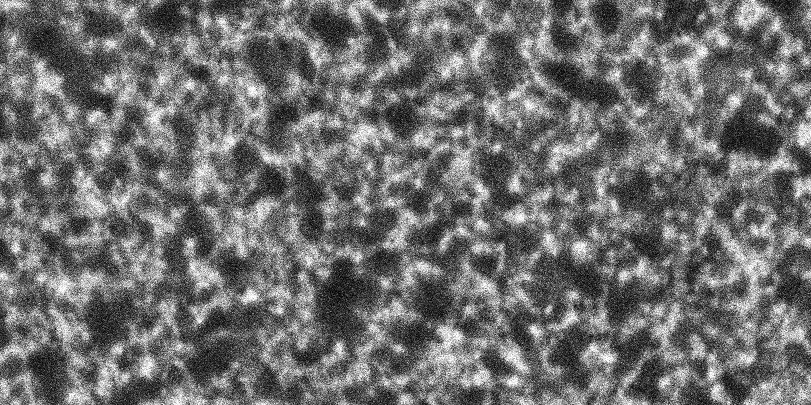
\includegraphics[width=3\TPHorizModule]{ech17_x63_time699_crop.jpg}\\
	\Subhead{Environmental SEM}\\
	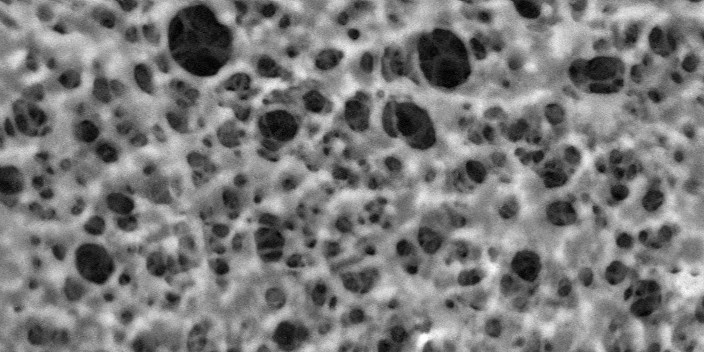
\includegraphics[width=3\TPHorizModule]{ESEM_cas4_GDL1-17_crop.jpg}\\
	\Subhead{Cryo SEM}\\
	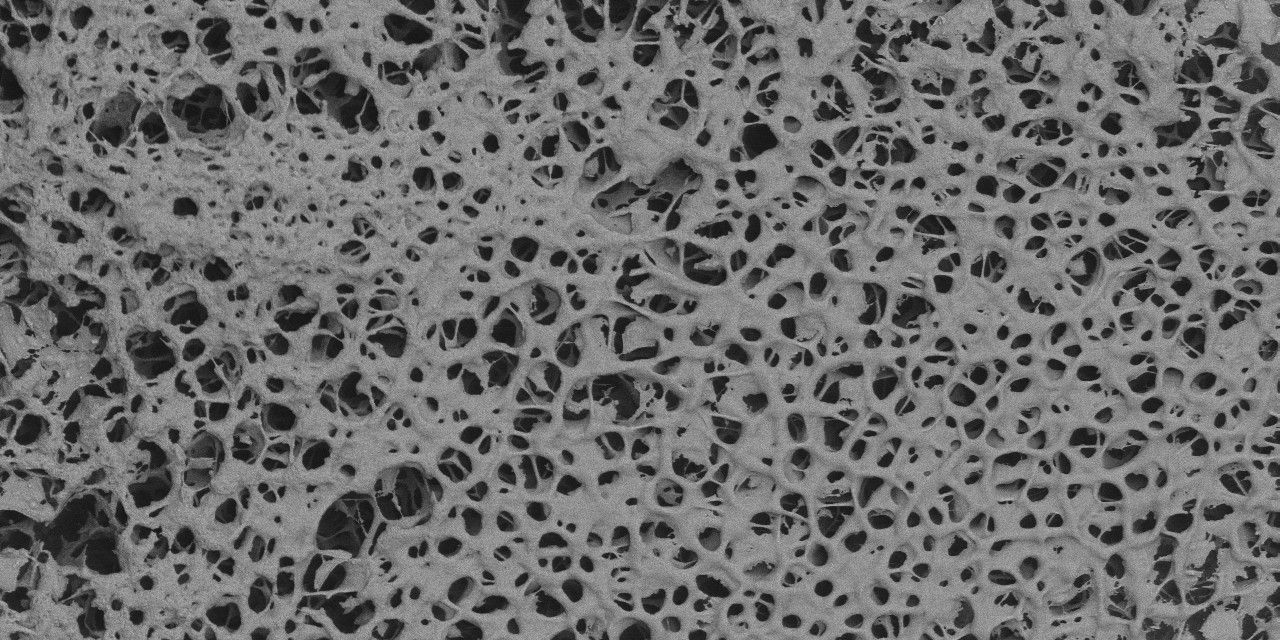
\includegraphics[width=3\TPHorizModule]{SEM_cas4_gdl1_22_crop.jpg}\\
};
\foreach \i in {2,4,6}
\draw[line width=0.2em, Accent2] (m-\i-1.south east) ++(-1em,1em) -- +(-0.75\TPHorizModule,0) node[midway, above] {\SI{10}{\micro\metre}};
\end{tikzpicture}

	
\end{textblock}

\begin{textblock}{11}(0,11.5)
	\Head{Evolution of the microscructure: preserved network, swelling aggregates}
	\tikzsetnextfilename{structure_confocal}
	\begin{tikzpicture}[every axis/.style={xlabel absolute, every axis x label/.append style={anchor=base, yshift=-1em}}]
\begin{groupplot}[
	group style={
			group name=g, group size=1 by 3,
			vertical sep=0.5em,
			xticklabels at=edge bottom,
		},
	scale only axis,
	height=3\baselineskip,
	width=3\TPHorizModule-3em,
	xmin=0, xmax=17, ymin=0,
	cycle list name=earthy,
	no marks,
	]
\nextgroupplot[ylabel={$\xi$ (\si{\micro\metre})}]
\addplot table[skip coords between index={0}{64}, x expr={\thisrowno{0}/3600}]{ech17_pore_size.txt};
\pgfplotsset{cycle list shift=4};
\addplot table[skip coords between index={0}{15}, x expr={\thisrowno{0}/3600}]{ech19_pore_size.txt};
\nextgroupplot[ylabel={$\chi$ (a.u.)}]
\begin{scope}[every node/.style={anchor=base west}]
\addplot table[skip coords between index={0}{64}, x expr={\thisrowno{0}/3600}, y expr={\thisrowno{2}/1e7}]{ech17_pore_size.txt} node (l1) {1\%};
\pgfplotsset{cycle list shift=4};
\addplot table[skip coords between index={0}{15}, x expr={\thisrowno{0}/3600}, y expr={\thisrowno{2}/1e7}]{ech19_pore_size.txt} node at ($(l1.base west)-(axis cs:0,1.8)$) {4\%};
\end{scope}
\nextgroupplot[xlabel={time (\si{\hour})}, ylabel={$\gamma$}]
\addplot table[skip coords between index={0}{64}, x expr={\thisrowno{0}/3600}, y index=3]{ech17_pore_size.txt};
\pgfplotsset{cycle list shift=4};
\addplot table[skip coords between index={0}{15}, x expr={\thisrowno{0}/3600}, y index=3]{ech19_pore_size.txt};
\end{groupplot}


\matrix[matrix of nodes, inner sep=0, row sep=0.2em, column sep=0.2em, matrix anchor=north west] 
at ($(g c1r1.right of north east)+(-11\TPHorizModule,0)$)
(m) {
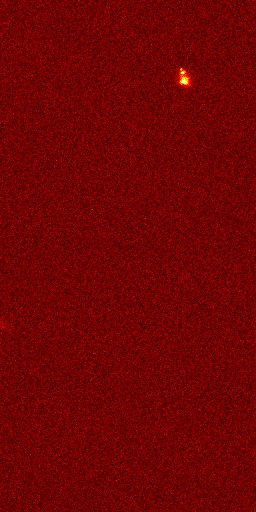
\includegraphics[width=5\baselineskip]{ech19_t001.jpg}&
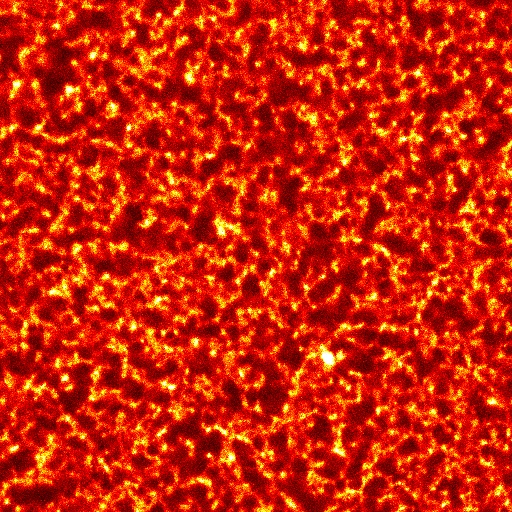
\includegraphics[width=5\baselineskip]{ech19_t043.jpg}&
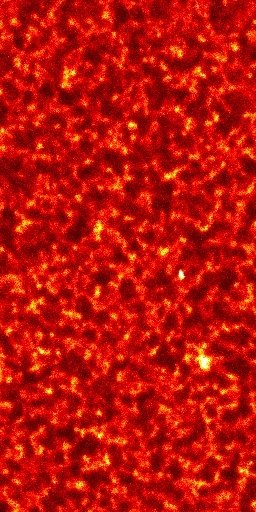
\includegraphics[width=5\baselineskip]{ech19_t085.jpg}&
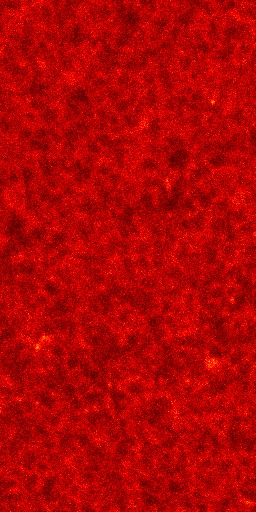
\includegraphics[width=5\baselineskip]{ech19_t132.jpg}\\
\SI{5}{\minute} & \SI{27}{\minute} & \SI{49}{\minute} & \SI{8}{\hour}\\
};
\draw[ultra thick, white] (m-1-1.south east) ++(-0.5\baselineskip,1em) -- +(-4\baselineskip,0) node[midway, above] {\SI{20}{\micro\metre}};

\newdimen\mydima
\newdimen\mydimb
\pgfextracty{\mydima}{\pgfpointanchor{g c1r1}{north}}
\pgfextracty{\mydimb}{\pgfpointanchor{g c1r3}{south}}
\begin{loglogaxis}[
	name=Sq,
	scale only axis,
	width=3\TPHorizModule,
	height=\mydima-\mydimb,
	anchor=left of north west,
	at={(m.north east)},
	cycle list name=earthy,
	xlabel={$q$ (\si{\per\micro\metre})},
	ylabel={$S(q)$ (a.u.)},
	domain=0.1:6.1,
	xmin=0.03, xmax=1e3,
	ymin=1e5, ymax=6e7,
	clip mode=individual,
	]
\begin{scope}[
	every axis plot post/.append style={only marks, mark options={scale=0.3}},
]
\addplot table{ech19_t016.Sq};
\addplot table{ech19_t018.Sq};
\addplot table{ech19_t020.Sq};
\addplot table{ech19_t022.Sq};
\addplot table{ech19_t024.Sq};
\addplot table{ech19_t026.Sq};
\addplot table{ech19_t028.Sq};

\pgfplotsset{cycle list shift=-7}
\addplot table[x expr={100*\thisrowno{0}}]{ech19_t049.Sq};
\addplot table[x expr={100*\thisrowno{0}}]{ech19_t091.Sq};
\addplot table[x expr={100*\thisrowno{0}}]{ech19_t095.Sq};
\addplot table[x expr={100*\thisrowno{0}}]{ech19_t110.Sq};
\addplot table[x expr={100*\thisrowno{0}}]{ech19_t132.Sq};
%\pgfplotsset{cycle list shift=2}
\addplot table[x expr={100*\thisrowno{0}}]{ech19_t183.Sq};
\end{scope}
\pgfplotsset{cycle list shift=-5}
\addplot+[domain=0.1:2.37] {1.54042e+06/(1+(0.830078*x)^(2.49725)} coordinate[pos=0] (t0);
\addplot+[domain=0.1:3.21] {3.18333e+06/(1+(0.674366*x)^(3.20292)};
\addplot+[domain=0.1:4.26] {7.33285e+06/(1+(0.682842*x)^(3.37189)};
\addplot+[domain=0.1:5.04] {1.30025e+07/(1+(0.683873*x)^(3.43697)};
\addplot+[domain=0.1:5.67] {2.02087e+07/(1+(0.681114*x)^(3.55135)};
\addplot+[domain=0.1:5.88] {2.69252e+07/(1+(0.674936*x)^(3.65006)};
\addplot+[domain=0.1:6.19] {3.16555e+07/(1+(0.67775*x)^(3.68483)} coordinate[pos=0] (t1);

\pgfplotsset{cycle list shift=-4}
\addplot+[domain=10:659.97] {3.95386e+07/(1+(0.0064764*x)^(3.88347)} coordinate[pos=0] (t2);
\addplot+[domain=10:607.05] {2.28285e+07/(1+(0.00584224*x)^(3.83587)};
\addplot+[domain=10:526.11] {1.43395e+07/(1+(0.00654421*x)^(3.73896)};
\addplot+[domain=10:454.51] {9.58685e+06/(1+(0.00865948*x)^(2.84983)};
\addplot+[domain=10:392.25] {6.8931e+06/(1+(0.00946977*x)^(2.56298)};
\addplot+[domain=10:373.57] {5.5388e+06/(1+(0.00950251*x)^(2.52804)} coordinate[pos=0] (t3);
\draw[->, line width=0.2em] (t0) -- (t1) node[midway,rotate=90, above] {time};
\draw[->, line width=0.2em] (t2) -- (t3) node[midway,rotate=90, above] {time};

\node[anchor=south west] at (rel axis cs:0,0) {$\displaystyle S(q) = \frac{\chi}{1+(\xi q)^\gamma}$};
\end{loglogaxis}
\end{tikzpicture}

	
\end{textblock}

\begin{textblock}{11}(0,15.5)
	\Head{Three creep regimes: much more chaotic when over-acidified}
	\tikzsetnextfilename{creep_cas4_gdl4}
	\begin{tikzpicture}
\pgfplotsset{every axis/.append style={xlabel absolute, every axis x label/.append style={anchor=base, yshift=-2em}, ylabel absolute, every axis y label/.append style={anchor=base, yshift=2em}}}
\begin{groupplot}[
	group style={
			group name=g, group size=4 by 1,
			horizontal sep=\TPHorizModule,
			%xticklabels at=edge bottom,
		},
	scale only axis,
	width=1.75\TPHorizModule,
	height=1.5\TPVertModule,
%	height=0.3\columnwidth-2em,
	cycle list name=earthy,
	xmode=log, ymode=log,
	%xmin=5e-2, xmax=1e3,
	ylabel={$\dot{\gamma}/\dot{\gamma}_\text{min}$},
	extra tick style={grid=major},%
	]
\nextgroupplot[
	xlabel={$t$ (\si{\second})}, ylabel={$\gamma$}, 
	ymax=3, ymin=2e-1,xmin=0.3,xmax=1e6,
	xtick={1, 1e2, 1e4, 1e6},
	ytick={0.1,0.2,0.4,0.8,1.6}, yticklabels={0.1,0.2,0.4,0.8,1.6},
	extra y ticks={1}, extra y tick labels={},]
\begin{scope}[every node/.style={, anchor=north west, inner xsep=0}]
\addplot table {Y242_20Pa_gamma_decimated.txt} node[pos=0.5, rotate=35] {\SI{20}{\pascal}};
\addplot table {Y239_40Pa_gamma_decimated.txt} node[pos=0.4, rotate=35] {\SI{40}{\pascal}};
\addplot table {Y238_50Pa_gamma_decimated.txt} node[anchor=south east, rotate=90] at (rel axis cs:0.78,1) {\SI{50}{\pascal}};
\addplot table {Y246_60Pa_gamma_decimated.txt} node[anchor=south east, rotate=90] at (rel axis cs:0.6,1) {\SI{60}{\pascal}};
\addplot table {Y236_100Pa_gamma_decimated.txt} node[pos=0.1, rotate=15] {\SI{100}{\pascal}};
\addplot+[restrict x to domain=0.05:100] table {Y249_120Pa_gamma_decimated.txt} node[anchor=north east, rotate=80] at (rel axis cs:0.15,1) {\SI{120}{\pascal}};
\end{scope}

\nextgroupplot[
	xlabel={$t/\tau_f$},xmin=1e-5, xmax=2, xtick={1e-4, 1e-2, 1},
	ymin=0.5, ymax=5e4]
\addplot table {Y242_20Pa_gdot_decimated.txt};
\addplot table {Y239_40Pa_gdot_decimated.txt};
\addplot table {Y238_50Pa_gdot_decimated.txt};
\addplot table {Y246_60Pa_gdot_decimated.txt};
\addplot table {Y236_100Pa_gdot_decimated.txt};
\addplot+[restrict x to domain=-2.75:1] table {Y249_120Pa_gdot_decimated.txt};
\node[below right] at (rel axis cs:0,1){Andrade creep};

\nextgroupplot[
	xlabel={$t/\tau_f$}, xmode=linear, ymode=linear, 
	xmin=0, xmax=1,ymin=0.5,ymax=10, restrict y to domain=0:11,
	xtick={0, 0.2, ..., 1}, ytick={2,4,6,8}]
\addplot table {Y242_20Pa_gdot_decimated.txt};
\addplot table {Y239_40Pa_gdot_decimated.txt};
\addplot table {Y238_50Pa_gdot_decimated.txt};
\addplot table {Y246_60Pa_gdot_decimated.txt};
\addplot table {Y236_100Pa_gdot_decimated.txt};
\addplot table {Y249_120Pa_gdot_decimated.txt};

\nextgroupplot[
	xlabel={$1-t/\tau_f$},xmin=1e-5, xmax=2, x dir=reverse, xtick={1e-4, 1e-2, 1},
	ymin=0.5, ymax=5e4]
\addplot table[x expr={1-\thisrowno{0}}] {Y242_20Pa_gdot_decimated.txt};
\addplot table[x expr={1-\thisrowno{0}}] {Y239_40Pa_gdot_decimated.txt};
\addplot table[x expr={1-\thisrowno{0}}] {Y238_50Pa_gdot_decimated.txt};
\addplot table[x expr={1-\thisrowno{0}}] {Y246_60Pa_gdot_decimated.txt};
\addplot table[x expr={1-\thisrowno{0}}] {Y236_100Pa_gdot_decimated.txt};
\addplot table[x expr={1-\thisrowno{0}}] {Y249_120Pa_gdot_decimated.txt};
\node[below right] at (rel axis cs:0,1){Finite time divergence};
\end{groupplot}
\node[inner sep=0] at ($(g c4r1.east)-(11\TPHorizModule,0)$) {};
\end{tikzpicture}
	
\end{textblock}

\begin{textblock}{3}(12,15.5)
	\Head{Monkman-Grant}
	Predict failure from the minimum
	
	\tikzsetnextfilename{MonkmanGrant}
	\begin{tikzpicture}
\pgfplotsset{every axis/.append style={
	xlabel absolute, every axis x label/.append style={anchor=base, yshift=-2em}, 
	ylabel absolute, every axis y label/.append style={anchor=base, yshift=2em},
	scale only axis,
	width=2\TPHorizModule,
	height=1.5\TPVertModule,
	xmode=log, xmin=1, xmax=1e6,
	domain=1:1e6,
}}
\begin{axis}[
	name=a,
	ylabel={$\tau_m$ (\si{\second})}, ymode=log, ymin=1,
	legend pos=north west,
	legend style={font=\scriptsize, fill=none, draw=none},
	xticklabels={}
]
\addplot[only marks, mark=*] table[x index=4, y index=5]{MCR_cas4_GDL1_gap10.txt};
\addlegendentry{1\%, $e=\SI{1}{\milli\metre},\, H=\SI{28}{\milli\metre}$};
\addplot[only marks, mark=square*] table[x index=4, y index=5]{MCR_cas4_GDL1_gap30.txt};
\addlegendentry{1\%, $e=\SI{3}{\milli\metre},\, H=\SI{28}{\milli\metre}$};
\addplot[gray, only marks, mark=o] table[x index=4, y index=5]{ARG2_cas4_GDL1_gap20.txt};
\addlegendentry{1\%, $e=\SI{1}{\milli\metre},\, H=\SI{60}{\milli\metre}$};
\addplot[red, only marks, mark=star] table[x index=4, y index=5]{MCR_cas4_GDL4_gap10.txt};
\addlegendentry{4\%, $e=\SI{1}{\milli\metre},\, H=\SI{28}{\milli\metre}$};
\addplot[no marks]{0.6*x};
\addplot[no marks, dashed]{0.4*x};
\end{axis}

\begin{axis}[
	anchor=north west,
	at={(0,-0.5em)},
	height=1\TPVertModule,
	xlabel={$\tau_f$ (\si{\second})},
	ylabel=$\tau_m/\tau_f$, ymin=0, 
]
\addplot[only marks, mark=*] table[x index=4, y expr={\thisrowno{5}/\thisrowno{4}}]{MCR_cas4_GDL1_gap10.txt};
\addplot[only marks, mark=square*] table[x index=4, y expr={\thisrowno{5}/\thisrowno{4}}]{MCR_cas4_GDL1_gap30.txt};
\addplot[gray, only marks, mark=o] table[x index=4, y expr={\thisrowno{5}/\thisrowno{4}}]{ARG2_cas4_GDL1_gap20.txt};
\addplot[red, only marks, mark=star] table[x index=4, y expr={\thisrowno{5}/\thisrowno{4}}]{MCR_cas4_GDL4_gap10.txt};
\addplot[no marks]{0.6};
\addplot[no marks, dashed]{0.4};
\end{axis}

%\node[inner sep=0] at ($(a.east)-(3\TPHorizModule,0)$) {};
\end{tikzpicture}
	
\end{textblock}

\begin{textblock}{11}(0,18.5)
	\Head{Basquin law rescaling}
	\begin{tabu}{XX}
	\Subhead{Composition} rescaled by elastic modulus&
	\Subhead{Geometry} rescaled as a fracture nucleation rate
	\end{tabu}	
	
	\tikzsetnextfilename{basquin}
	\begin{tikzpicture}
\pgfplotsset{every axis/.append style={xlabel absolute, every axis x label/.append style={anchor=base, yshift=-2em}, ylabel absolute, every axis y label/.append style={anchor=base, yshift=2em}}}
\begin{groupplot}[
	group style={
			group name=g, group size=4 by 1,
		   % group name=g, group size=2 by 2,
		   horizontal sep=\TPHorizModule,
			vertical sep=3.5em,
%			xticklabels at=edge bottom,
			%y descriptions at=edge left,
		},
	scale only axis,
	width=1.75\TPHorizModule,
	xmode=log, ymode =log,
	ymax=2e6, xmin=0.125, xmax=2,
	xlabel=$\sigma/G^\prime$,
	ylabel={$\tau_\text{min}$ (\si{\second})},
	cycle list name=earthy,
	clip mode=individual,
	%cycle list shift=2,
	%ymin=0.01, ymax=1e6,
%	xmin=0, xmax=17, ymin=0,
%	cycle list name=linestyles,
%	no marks,
	]

%composition
\nextgroupplot[xlabel={$\sigma$ (\si{\pascal})}, xmin=10, xmax=2e3, ymin=2e-2, ytickten={-1,1,3,5}]
%\pgfplotsset{cycle list shift=3}
\addplot+[only marks, mark=square*] table[y index=5]{MCR_cas4_GDL1_gap10.txt} node[midway, above right] {1\%};
\addplot+[only marks, mark=square, black] table[y index=5]{MCR_cas4_GDL4_gap10.txt} node[midway, above right] {4\%};
%fits
\addplot[gray, domain=150:1000] {3.7e17*x^(-5.5)};
\addplot[gray, domain=20:350] {3.7e12*x^(-5.5)};

%composition rescaled
\nextgroupplot[xmax=4, ymin=2e-2, xtick={0.25, 0.5, 1, 2,4}, xticklabels={0.25, 0.5, 1, 2,4}, ytickten={-1,1,3,5}]
\addplot+[only marks, mark=square*] table[x expr={\thisrowno{0}/\thisrowno{2}}, y index=5]{MCR_cas4_GDL1_gap10.txt};
\addplot+[only marks, mark=square, black] table[x expr={\thisrowno{0}/\thisrowno{2}}, y index=5]{MCR_cas4_GDL4_gap10.txt};
%fit
\addplot[gray, domain=0.18:3.5] {40.6*x^(-5.5)} node[midway, below left] {-5.5};

%gap
\nextgroupplot[xtick={0.25, 0.5, 1}, xticklabels={0.25, 0.5, 1}, ymin=8]
%\addplot+[only marks] table[x expr={\thisrowno{0}/\thisrowno{2}}, y index=5]{MCR_cas4_GDL1_gap05.txt};
%\pgfplotsset{cycle list shift=2}
\addplot+[only marks, mark=square*] table[x expr={\thisrowno{0}/\thisrowno{2}}, y index=5]{MCR_cas4_GDL1_gap10.txt} node[pos=0, above right] {$e=\SI{1}{\milli\metre}$};
\pgfplotsset{cycle list shift=2}
\addplot+[only marks, mark=diamond*] table[x expr={\thisrowno{0}/\thisrowno{2}}, y index=5]{MCR_cas4_GDL1_gap15.txt} node (los){} node[above left] (lablos) at (rel axis cs:1, 0.6) {$e=\SI{1.5}{\milli\metre}$} [->] (lablos.base west) -| (los);
\pgfplotsset{cycle list shift=4}
\addplot+[only marks, mark=*] table[x expr={\thisrowno{0}/\thisrowno{2}}, y index=5]{MCR_cas4_GDL1_gap30.txt} node[below left] at (axis cs:0.5,1e2){$e=\SI{3}{\milli\metre}$};
%fit
\addplot[gray, domain=0.2:1.3] {40.6*x^(-5.5)};
\addplot[gray, domain=0.17:0.5] {0.77*x^(-5.5)};

%gap rescaled
\nextgroupplot[ylabel={$\tau_\text{min} e^3$ (\si{\cubic\milli\metre\second})},xtick={0.25, 0.5, 1}, xticklabels={0.25, 0.5, 1}, ymin=8]
%\addplot+[only marks] table[x expr={\thisrowno{0}/\thisrowno{2}}, y expr={\thisrowno{5}*0.5^3}]{MCR_cas4_GDL1_gap05.txt};
%\pgfplotsset{cycle list shift=2}
\addplot+[only marks, mark=square*] table[x expr={\thisrowno{0}/\thisrowno{2}}, y expr={\thisrowno{5}*1^3}]{MCR_cas4_GDL1_gap10.txt};
\pgfplotsset{cycle list shift=2}
\addplot+[only marks, mark=diamond*] table[x expr={\thisrowno{0}/\thisrowno{2}}, y expr={\thisrowno{5}*1.5^3}]{MCR_cas4_GDL1_gap15.txt};
\pgfplotsset{cycle list shift=4}
\addplot+[only marks, mark=*] table[x expr={\thisrowno{0}/\thisrowno{2}}, y expr={\thisrowno{5}*3^3}]{MCR_cas4_GDL1_gap30.txt};
%fit
\addplot[gray, domain=0.15:1.3] {34.9*x^(-5.5)};

\end{groupplot}
\node[inner sep=0] at ($(g c4r1.east)-(11\TPHorizModule,0)$) {};
\end{tikzpicture}
	
\end{textblock}

\begin{textblock}{3}(12,20)
	\Head{Wavelength}
	\tikzsetnextfilename{lambda}
	\begin{tikzpicture}
%\pgfplotsset{every axis/.append style={xlabel absolute, every axis x label/.append style={anchor=base, yshift=-2em}, ylabel absolute, every axis y label/.append style={anchor=base, yshift=2em}}}
\begin{groupplot}[
	group style={
			group name=g, group size=1 by 2,
			vertical sep=3.25em,
%			xticklabels at=edge bottom,
			%y descriptions at=edge left,
		},
	scale only axis,
	width=2\TPHorizModule,
	height=1\TPVertModule,
	xmin=0, ymin=0,
	ylabel={$\lambda$ (\si{\milli\metre})},
]

\nextgroupplot[xlabel={$\sigma$ (\si{\pascal})}, xmax=900, xtick={0,200,...,800}]
\addplot[only marks, error bars/.cd, y dir=both, y explicit] table[y error=erreur]{lambda_sigma_cas4_GDL1_ARG2.txt};
\addplot[mark=o, only marks, error bars/.cd, y dir=both, y explicit] table[y error=erreur]{lambda_sigma_cas4_GDL4_ARG2.txt};
\addplot[no marks, domain=0:900] {2.61};
\addplot[no marks, dotted, domain=0:900] {3.25};

\nextgroupplot[xlabel={gap (\si{\milli\metre})}, xmax=3.5, cycle list name=earthy]
\addplot[mark=o, only marks, error bars/.cd, y dir=both, y explicit] table[x=gap, y=lambda, y error=erreur, restrict expr to domain={\thisrowno{0}}{20:26}]{lambda_gap_cas4GDL4.txt};
\addplot+[mark=*, only marks, error bars/.cd, y dir=both, y explicit] coordinates{(2,2.61) +- (0,0.34)};
\pgfplotsset{cycle list shift=2};
\addplot+[mark=diamond*, only marks, error bars/.cd, y dir=both, y explicit] table[x=gap, y=lambda, y error=erreur, restrict expr to domain={\thisrowno{0}}{30:38}]{lambda_gap_cas4GDL4.txt};
\pgfplotsset{cycle list shift=3};
\addplot+[mark=triangle*, only marks, error bars/.cd, y dir=both, y explicit] table[x=gap, y=lambda, y error=erreur, restrict expr to domain={\thisrowno{0}}{38:50}]{lambda_gap_cas4GDL4.txt};
\addplot[no marks, domain=0:4] {1.3*x};
%\addplot[only marks, error bars/.cd, y dir=both, y explicit] table[x=gap, y expr={\thisrow{lambda}}, y error=erreur]{lambda_gap_cas4GDL1.txt};

\end{groupplot}
\newdimen\mydima
\pgfextractx{\mydima}{\pgfpointanchor{g c1r1}{north east}}
\node[inner sep=0, above left =0.5em and 0 of g c1r1.north east] (im) {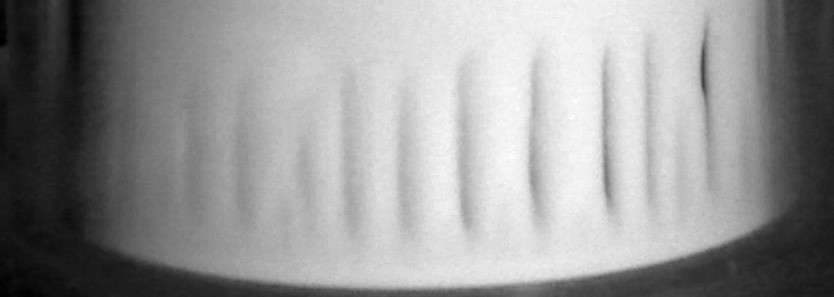
\includegraphics[width=\mydima]{Y140_bottom}};
\draw[<->] (im.north west) ++ (0.48\mydima, -0.2\mydima) -- +(0.075\mydima,0) node[midway,above] {$\lambda$};

\end{tikzpicture}

	
\end{textblock}

\begin{textblock}{15}(0,24.75)
\small{\texttt{The research leading to these results has received funding from the European Research Council under the European Union's Seventh Framework Programme (FP7/2007-2013) / ERC grant agreement n°~258803.}}
\end{textblock}


\textblockcolour{lightgray!50!white}
\TPMargin*{ 0.125\TPHorizModule }
\begin{textblock}{2.875}(12,3.125)%real width of 3
	\Norulehead{Take home}
	Spontaneous wrinkling of over-acidified casein gels in non-adhesive confinement
	
	\Subhead{Original patterns}
	\begin{itemize}
		\item nested (optical elements ?)
		\item kinetic wavelength selection
	\end{itemize}
	\Subhead{A new wrinkling mechanism}
	\begin{itemize}
		\item porous flow resist bending
		\item Darcy can beat Poiseuille
		\item may extend to other porous sheets\linebreak  (wet paper, biological membranes\ldots)
	\end{itemize}
	\Subhead{Viscosity influences}
	\begin{itemize}
		\item porous dissipation
		\item gel formation\hfill
		\raisebox{0.6\normalbaselineskip}[0pt][0pt]{$\left.\rule{0pt}{1.1\normalbaselineskip}\right\}$ thus wrinkling}
	\end{itemize}
	

\end{textblock}%Conclusion



\end{document}